\chapter{Host Organization \& Internship Context}
\label{chap:host-organization}

% ═════════════════════════════════════════════════════════════
\section{\textcolor[HTML]{0066CC}{Organization Overview}}
\label{sec:org-overview}
% ═════════════════════════════════════════════════════════════

\subsection*{\textcolor[HTML]{003D99}{2.1.1 Groupe Stellantis: Creation and Scope}}

\textbf{Stellantis} is a multinational automotive group that has arisen from the merger of \textbf{Groupe PSA} and \textbf{Fiat Chrysler Automobiles (FCA)}, since the \textbf{January 16, 2021}. 
The group operates globally, and in addition has responsibility for a vast number of different car brands in such areas as passenger vehicles, SUVs and commercial vehicles.

\begin{figure}[!htbp]
  \centering
  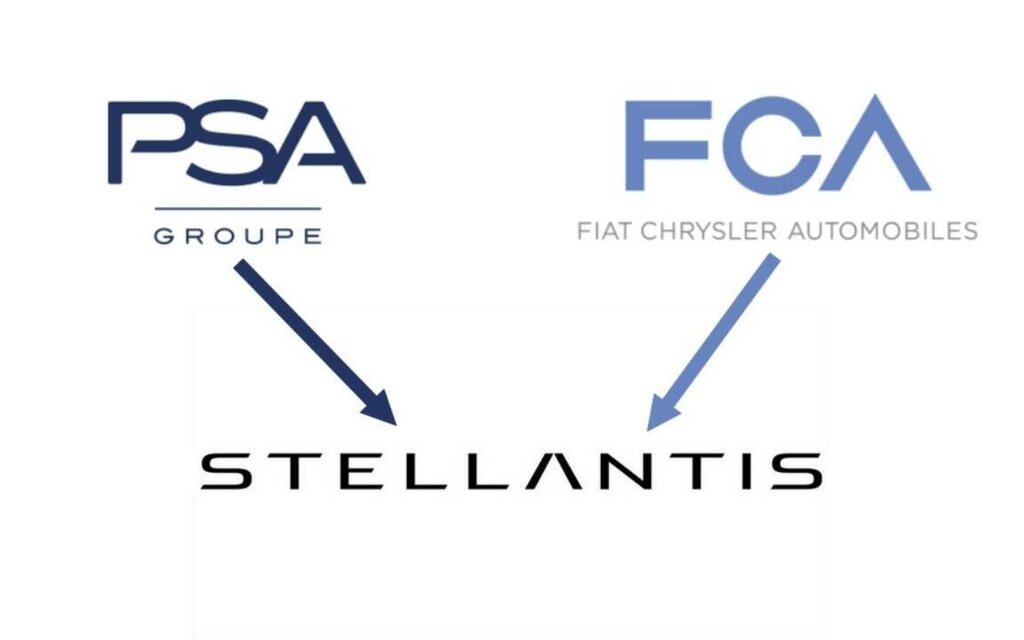
\includegraphics[width=0.75\textwidth]{images_pfe/psa fca.jpg}
  \caption{Formation of Stellantis through Groupe PSA and FCA merger (effective January 16, 2021).}
  \label{fig:psa_fca_merger}
\end{figure}


The group structure brings together industry, engineering and technology development across the group sites. Actually, this group structure makes it possible for Stellantis to organize vehicles design, parts and volume production under a unified framework.
\begin{figure}[!htbp]
  \centering
  
\includegraphics[width=0.75\textwidth]{images_pfe/mark.jpg}
  \caption{Stellantis automotive brands portfolio (represents multi-brand governance structure).}
  \label{fig:stellantis brands}
\end{figure}
\vspace{0.3cm}

\subsection*{\textcolor[HTML]{003D99}{2.1.2 Sochaux Site: Historical Context and Current Production}}

The conducted internship took place in the\textbf{Sochaux manufacturing facility}. A plant located in the eastern of the France. This plant represents a large number of historical plants for the group Stellantis as the producing operation run during an alternate period since \textbf{1912}, during the initial Peugeot ownership. At this day, the plant has a major goal to produce multi-energy SUVs as the \textbf{Peugeot 3008} and \textbf{5008} models. According to the renewal plan, it has been designed again and aimed in the future to become a forward engineering and producing plant.

\begin{figure}[!htbp]
  \centering
  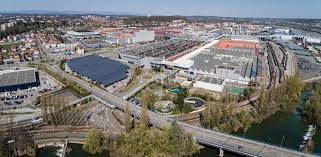
\includegraphics[width=0.75\textwidth]{images_pfe/stellantis.jpg}
  \caption{Sochaux Plant of Stellantis.}
  \label{fig:sochaux_plant}
\end{figure}

\FloatBarrier

% ═════════════════════════════════════════════════════════════
\section{\textcolor[HTML]{0066CC}{Organizational Structure and Interfaces}}
\label{sec:org-structure}
% ═════════════════════════════════════════════════════════════

\subsection*{\textcolor[HTML]{003D99}{2.2.1 Mechatronics Engineering: Mission and Scope}}

The internship was performed within the \textbf{Mechatronics Engineering Department} of the Sochaux site. Mechatronics is the integrated engineering which need to join three domains:
{\setlength{\intextsep}{6pt}
\begin{figure}[H]
  \centering
  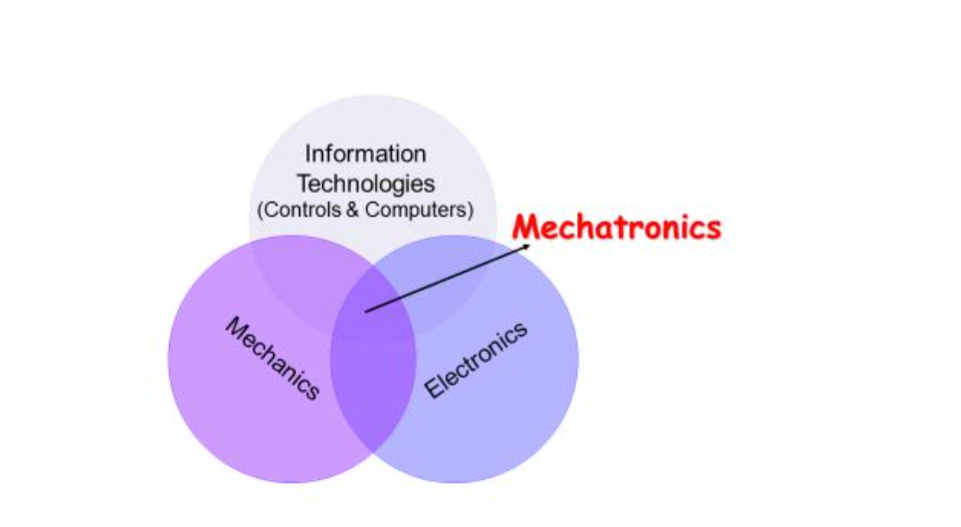
\includegraphics[width=0.75\textwidth]{images_pfe/mechatronics.png}
  \caption{Mechatronics Engineering Department Overview.}
  \label{fig:mechatronics_overview}
\end{figure}
}
\FloatBarrier
\vspace{-4pt}

It is the Mechatronics department that provides a high contribution to the systems evolution of the vehicle within the Stellantis program framework, making sure the three domains are working together providing advanced engineering system solutions for the automotive world. 
The department, together with System Engineering, Component Engineering and Project Management, guarantees the execution of all schedule and Technology Readiness levels deliverables (Gates 1, 2, 3 gates).
\vspace{0.3cm}

\subsection*{\textcolor[HTML]{003D99}{2.2.2 Key Stakeholder Roles in Governance}}

There are 4 main functions involved in Sochaux management, each has a precise task to be carried out within the component validation and gate release process. Those can be summarised as below:
\vspace{0.3cm}


\begin{table}[H]
\centering
\small
\setlength{\tabcolsep}{8pt}
\renewcommand{\arraystretch}{2.2}
\caption{Governance roles and responsibilities at Sochaux Mechatronics.}
\label{tab:governance-roles}
\begin{tabularx}{\textwidth}{|>{\raggedright\arraybackslash}X|>{\raggedright\arraybackslash}X|>{\raggedright\arraybackslash}X|}
\hline
\cellcolor[HTML]{E6F2FF}\textcolor[HTML]{003D99}{\textbf{Role}} & \cellcolor[HTML]{E6F2FF}\textcolor[HTML]{333333}{\textbf{Responsibilities}} & \cellcolor[HTML]{E6F2FF}\textcolor[HTML]{006600}{\textbf{Interactions \& Data Sources}} \\
\hline
\textbf{DL}\newline(Design Leader) & Technical ownership, Specification definition, PM coordination & Who-is-Who Excel entry, specification delivery, blocker escalation to PM \\
\hline
\textbf{DRE}\newline(Design Review Engineer) & Design review execution, Compliance verification, Gate readiness assessment & Specification review, gate criteria validation, documentation flagging \\
\hline
\textbf{CTE}\newline(Chief Technical Expert) & Multi-component support, Standards guidance, Conflict arbitration & On-demand technical advice, standards compliance, DL--DRE escalation point \\
\hline
\textbf{SSTL}\newline(Supplier Lead) & Supplier interface, Deliverable validation, Escalation path & Supplier communication, documentation validation, blocker escalation \\
\hline
\end{tabularx}
\end{table}

\vspace{0.2cm}


\noindent\textbf{Decision and Escalation Pathways:}

\vspace{0.3cm}

\fbox{\begin{minipage}{0.92\textwidth}

\small

\noindent\textcolor[HTML]{003D99}{\textbf{1. Routine Approval}} \quad $\Rightarrow$ DL \& DRE consensus required

\vspace{0.1cm}

\hspace{0.5cm} • Both actors aligned \quad $\Rightarrow$ \textcolor[HTML]{006600}{\textbf{Gate Progression}} 

\vspace{0.3cm}

\noindent\textcolor[HTML]{CC6600}{\textbf{2. Technical Disputes}} \quad $\Rightarrow$ CTE provides expert arbitration

\vspace{0.1cm}

\hspace{0.5cm} • If resolved \quad $\Rightarrow$ \textcolor[HTML]{006600}{\textbf{Decision}} 

\vspace{0.1cm}

\hspace{0.5cm} • If unresolved \quad $\Rightarrow$ \textcolor[HTML]{CC0000}{\textbf{Escalate to PM}}

\vspace{0.3cm}

\noindent\textcolor[HTML]{CC0000}{\textbf{3. Supplier Issues}} \quad $\Rightarrow$ SSTL manages supplier interface

\vspace{0.1cm}

\hspace{0.5cm} • If resolved \quad $\Rightarrow$ \textcolor[HTML]{006600}{\textbf{Decision}} 

\vspace{0.1cm}

\hspace{0.5cm} • If unresolved \quad $\Rightarrow$ \textcolor[HTML]{CC0000}{\textbf{Escalate to PM}}

\end{minipage}}

\FloatBarrier

% ═════════════════════════════════════════════════════════════
\section{\textcolor[HTML]{0066CC}{Department and Project Context}}
\label{sec:dept-context}
% ═════════════════════════════════════════════════════════════

\subsection*{\textcolor[HTML]{003D99}{2.3.1 Engineering Governance Processes}}

The governance in Sochaux is a cyclical approach (preparation/review/decision) related to milestones of the technical solution. These parts are governed by maturity gates (Gate 1, Gate 2, Gate 3), and involve creation, validation and approval of deliverables. This process includes teams of engineers (DL, DRE) and managers (PM, CTE), with well defined decisions taken, recorded and referenced.
\vspace{0.3cm}

\noindent\textbf{Governance Workflow:}

\begin{table}[!htbp]
\centering
\footnotesize
\setlength{\tabcolsep}{4pt}
\renewcommand{\arraystretch}{1.6}
\caption{Engineering Governance Workflow at Sochaux}
\begin{tabularx}{\textwidth}{|>{\raggedright\arraybackslash}p{1.55cm}|>{\raggedright\arraybackslash}p{1.5cm}|>{\raggedright\arraybackslash}p{2.05cm}|>{\raggedright\arraybackslash}p{2.1cm}|>{\raggedright\arraybackslash}p{1.8cm}|>{\raggedright\arraybackslash}p{1.8cm}|>{\raggedright\arraybackslash}p{1.85cm}|}
\hline
\textcolor[HTML]{003D99}{\textbf{Step}} & \textcolor[HTML]{003D99}{\textbf{Actor}} & \textcolor[HTML]{003D99}{\textbf{Action}} & \textcolor[HTML]{003D99}{\textbf{Inputs}} & \textcolor[HTML]{003D99}{\textbf{Outputs}} & \textcolor[HTML]{003D99}{\textbf{Decision}} & \textcolor[HTML]{003D99}{\textbf{Tools}} \\
\hline
Alignment & DL, PM & Discuss status, identify blockers & Project plan, task list & Current state & Proceed / escalate & Excel, SharePoint \\
\hline
Review & DRE & Inspect deliverables & Specifications, reports & Validation report & Accept / reject & SharePoint \\
\hline
Validation & DRE, DL & Check compliance & Deliverables & Compliance result & Approve / correct & SharePoint \\
\hline
Gate Decision & DL, DRE & Approve component status & Validation report & Approval & Gate pass / escalate & SharePoint, email \\
\hline
Escalation & CTE, PM & Resolve technical disputes & Issues & Solution & Resolution & Meetings, email \\
\hline
\end{tabularx}
\label{tab:governance-workflow}
\end{table}

\vspace{0.3cm}

\noindent\textbf{Process Flow:}

\vspace{0.3cm}

\noindent\fbox{\begin{minipage}{0.92\textwidth}
\centering
\small
\textcolor[HTML]{003D99}{\textbf{DL}} $\Rightarrow$ creates and uploads deliverables

\vspace{0.2cm}

\quad\quad\quad\quad\quad $\Downarrow$

\vspace{0.1cm}

\textcolor[HTML]{003D99}{\textbf{DRE}} $\Rightarrow$ reviews against gate requirements

\vspace{0.2cm}

\begin{tabular}{ll}
\quad\quad\quad\quad\quad $\Downarrow$ & \\
\end{tabular}

\vspace{0.1cm}

If \textcolor[HTML]{006600}{\textbf{validated}} $\Rightarrow$ \textcolor[HTML]{006600}{\textbf{gate progression approved}}

If \textcolor[HTML]{CC0000}{\textbf{issues}} $\Rightarrow$ \textcolor[HTML]{CC0000}{\textbf{DL applies corrections}}

If \textcolor[HTML]{FF6600}{\textbf{conflict}} $\Rightarrow$ \textcolor[HTML]{FF6600}{\textbf{escalation to CTE / PM}}

\end{minipage}}

\vspace{0.3cm}

\noindent\textbf{Gate Status Determination:}

Gate progression is tracked by looking at whether the document is available and is validated in SharePoint, not on a centralized system. The progression steps are as follows:
\vspace{0.3cm}

\begin{table}[H]
\centering
\small
\setlength{\tabcolsep}{8pt}
\renewcommand{\arraystretch}{2.2}
\caption{Gate Progression Requirements at Sochaux Mechatronics.}
\label{tab:gate-progression}
\begin{tabularx}{\textwidth}{|>{\raggedright\arraybackslash}X|>{\raggedright\arraybackslash}X|>{\raggedright\arraybackslash}X|}
\hline
\cellcolor[HTML]{E6F2FF}\textcolor[HTML]{003D99}{\textbf{Gate 1}} & \cellcolor[HTML]{E6F2FF}\textcolor[HTML]{003D99}{\textbf{Gate 2}} & \cellcolor[HTML]{E6F2FF}\textcolor[HTML]{003D99}{\textbf{Gate 3}} \\
\hline
Specification approved and uploaded & Design report completed + Design Review closed & Test reports + Compliance certificates available \\
\hline
\end{tabularx}
\end{table}

\vspace{0.2cm}

\noindent This is a document based system and, as such, is flexible; but care must be taken to monitor the system, as data can become disparate or inconsistent.

\vspace{0.3cm}

\noindent\textbf{Integration with LEON:}

Based on the requirements identified for this specific model of operational governance (manual sync, document correctness and decentralized data sources) there is a need for a system which will provide easy access to governance information and automate these requirements. A system capable of fulfilling these requirements (LEON) is described in the following sections.

\subsection*{\textcolor[HTML]{003D99}{2.3.2 Current Challenges in Governance Operations}}

Three persistent challenges constrain governance effectiveness at Sochaux:

\vspace{0.2cm}

\noindent\textbf{1. Information Fragmentation}

All the governance data (roles, status of gates, deliverables) are located in separated places: in an Excel spreadsheet stored on a SharePoint site, in a project portal database and in an e-mail sheet archives. If an engineer would like to know who is DRE for a given component, the following procedure should be performed: enter in project directory, search the right responsibility spreadsheet, locate the component, analyze the role columns. It could take from 10 seconds to one hour depending on the sheet condition.
\vspace{0.2cm}

\noindent\textbf{2. Data Inconsistency}

It is possible for a component to have different DLs or DREs on different Excel spreadsheets (example across projects, or at different times on the same project due to the changing of responsibility). If there is no single source of truth, the stakeholders have no means of knowing which data is the most current, and the teams sit around waiting for decision and approval of rework.
\vspace{0.2cm}

\noindent\textbf{3. Manual Coordination Overhead}

At each review / gate decision, this action is manually executed: collect data (check state of deliverable by person in charge, check for conformingness). As many projects running in parallel, and several elements within a project to manage, this overhead increases exponentially.
\FloatBarrier

% ═════════════════════════════════════════════════════════════
\section{\textcolor[HTML]{0066CC}{Internship Scope and Deliverables}}
\label{sec:internship-scope}
% ═════════════════════════════════════════════════════════════

\vspace{0.3cm}

\subsection*{\textcolor[HTML]{003D99}{2.4.1 Genesis of LEON: Addressing Governance Challenges}}

It is intended that \textbf{\textcolor[HTML]{0066CC}{LEON}} will be a governance support tool that will centralize a lot of consumed distributed governance information (e.g. roles, gate status) and be able to answer questions quickly. The tool will access existing storage location (SharePoint, Excel spreadsheet) and deliver information through natural language in no waiting for search.

\vspace{0.2cm}

\noindent\textbf{Scope and Intent:}

LEON is not intended as a replacement for governance process validation, gate decisions, or compliance checks. They are carried out by human stakeholders (DL, DRE, CTE, PM). LEON helps to share information and coordinate in order to help engineers do the actual technical decisions rather than information retrieval.
\vspace{0.2cm}

\noindent\textbf{Addressing the Challenges:}

\begin{table}[!htbp]
\centering
\small
\setlength{\tabcolsep}{8pt}
\renewcommand{\arraystretch}{1.8}
\caption{How LEON Addresses Governance Challenges}
\begin{tabularx}{\textwidth}{|>{\raggedright\arraybackslash}X|>{\raggedright\arraybackslash}X|}
\hline
\cellcolor[HTML]{E6F2FF}\textcolor[HTML]{003D99}{\textbf{Challenge}} & \cellcolor[HTML]{E6F2FF}\textcolor[HTML]{003D99}{\textbf{LEON Contribution}} \\
\hline
Information Fragmentation & Centralizes Who-is-Who and gate status data from distributed repositories into single queryable source \\
\hline
Data Inconsistency & Enforces single version of authority with audit trail; stakeholders access same data \\
\hline
Manual Coordination Overhead & Enables instant response to routine queries (role lookup, gate status) without manual search cycles \\
\hline
\end{tabularx}
\label{tab:leon-challenges}
\end{table}

The next chapter deals with the technical design and the prototype implementation of LEON to fulfill the requirements stated.
\FloatBarrier

Work on the LEON prototype was done in three parallel work packages analysis (of the system‘s requirements), implementation (on the hardware) and validation (using representative scenarios).
\vspace{0.5cm}

\subsection*{\textcolor[HTML]{003D99}{2.4.2 Work Package 1 (WP1): Requirements Elicitation and Specification}}

\noindent\textbf{Objective} : Identify and list recurring major governance questions as well as the technical requirements.

\vspace{0.2cm}

\noindent\textbf{Activities} : Conducted stakeholder (DLs, DREs, PMs) interviews to collect usual questions and blockers in their processes. Collecting essential functions such as knowledge Who-is-Who, gate status, document check. Documented constraints are roles of access, data compliance and usabilty.

\vspace{0.2cm}

\noindent\textbf{Deliverables} : Reporting of requirements specification, user scenario catalog, system context diagram.

\vspace{0.5cm}

\subsection*{\textcolor[HTML]{003D99}{2.4.3 Work Package 2 (WP2): System Design and Prototype Implementation}}

\noindent\textbf{Objective} : To develop and deploy a working prototype onto the Stellantis enterprise systems.

\vspace{0.2cm}

\noindent\textbf{Activities} : Designed a system architecture that meets the requirements using the available enterprise tools (conversation engine, workflow orchestration, integrate with SharePoint and Excel tools). Implemented system functionality (Who-is-Who in excel, Infer deliverable status based on sharepoint gates, role based access etc..). Configured SharePoint integration.

\vspace{0.2cm}

\noindent\textbf{Deliverables} : System architecture documents, implementation manual, deployment kit for prototype.

\vspace{0.5cm}

\subsection*{\textcolor[HTML]{003D99}{2.4.4 Work Package 3 (WP3): Evaluation and Scenario-Based Testing}}

\noindent\textbf{Objective} : Verification of operation and applicability for real world use.

\vspace{0.2cm}

\noindent\textbf{Activities} : Prototype has been implemented to simulate test environment considering normal governance use cases. Conducted functional tests with reference to user journeys, correctness check of role lookup and gate status inference, correctness check of access control enforcement.

\vspace{0.2cm}

\noindent\textbf{Deliverables} : Test report, performance assessment, security assessment, feedback from stakeholders, recommendation to production



% ═════════════════════════════════════════════════════════════
\section{\textcolor[HTML]{0066CC}{Problem Definition \& Objectives}}
\label{sec:problem-objectives}
% ═════════════════════════════════════════════════════════════

\subsection{\textcolor[HTML]{003D99}{Problem Definition}}
\label{subsec:problem-def}

\subsubsection*{\textcolor[HTML]{003D99}{Central Problem Statement}}

The Mechatronics department at Sochaux faces a permanent operational difficulty: \textbf{the governance information required to answer common engineering questions (role, state of the gate, condition of compliance ...) is distributed in various systems and storage spaces, causing coordination effort and incoherence of the governance solution.}.

\vspace{0.3cm}

\subsubsection*{\textcolor[HTML]{003D99}{Root Causes and Symptoms}}

Team members (DL, DRE, CTE, SSTL) expect rapid and specific answers regarding normal governance problems. Currently, it is necessary to do a long (manual) search in the infrastructure:

\vspace{0.2cm}

\begin{table}[!htbp]
\centering
\small
\setlength{\tabcolsep}{8pt}
\renewcommand{\arraystretch}{2.1}
\caption{Governance Information Needs and Current Barriers}
\begin{tabularx}{\textwidth}{|>{\raggedright\arraybackslash}X|>{\raggedright\arraybackslash}X|>{\raggedright\arraybackslash}X|}
\hline
\cellcolor[HTML]{E6F2FF}\textcolor[HTML]{003D99}{\textbf{Question Needed}} & \cellcolor[HTML]{E6F2FF}\textcolor[HTML]{003D99}{\textbf{Current Process}} & \cellcolor[HTML]{E6F2FF}\textcolor[HTML]{003D99}{\textbf{Barriers}} \\
\hline
``Who is responsible for component X in role Y?'' & Manual Excel search, cross-reference sheets & Multiple sources, outdated data \\
\hline
``What is gate status of component Z?'' & Check SharePoint folder, infer from documents & No centralized metadata \\
\hline
``Is documentation meeting gate requirements?'' & Engage expert for manual review & Delays, inconsistent interpretation \\
\hline
\end{tabularx}
\label{tab:information-needs}
\end{table}

\vspace{0.3cm}

\subsubsection*{\textcolor[HTML]{003D99}{LEON's Value Proposition}}

\textbf{\textcolor[HTML]{0066CC}{LEON}} is proposed as a unified governance agent that:

\begin{itemize}
  \item \textbf{Centralizes access} to the right governance information (roles, gates, templates, rules on compliance).
  \item \textbf{Automates routine queries} to take some part of coordination load away, as well as shorten response time.
  \item \textbf{Enforces consistency} through centralized control and use of role-based access.
  \item \textbf{Provides traceability} of all governance decisions and actions to the extent required to comply with an audit.
  \item \textbf{Preserves human oversight} by including human validation and an escalation mechanism within it for critical decisions.
\end{itemize}

\FloatBarrier

\subsection{\textcolor[HTML]{003D99}{System Constraints and Design Drivers}}
\label{subsec:constraints}

\textbf{\textcolor[HTML]{0066CC}{LEON}} is implemented under certain enterprise constraints which is typical for the majority of industrial engineering type work environment. Due to that internal repositories must be made available to the users by role in order to avoid that governance data is exposed to everybody. Confidentiality constraints also prevent unreserved access to the information details which is contained in disclosed tools. The accountability of all access can support system auditing and the existence of LEON as a support rather than decision support can be regarded as being advantageous for the human decision makers.

\FloatBarrier

\subsection{\textcolor[HTML]{003D99}{Objectives and Success Criteria}}
\label{subsec:objectives}

\subsubsection*{\textbf{\textcolor[HTML]{0066CC}{Primary Objective}}}

Design and deliver a prototype governance agent that centralizes access to authoritative governance information and enables team members to obtain accurate answers to recurring governance questions through natural language conversation, while maintaining strict role-based access control and auditability.

\vspace{0.5cm}

\subsubsection*{\textbf{\textcolor[HTML]{0066CC}{Measurable Sub-Objectives and Success Criteria}}}

\begin{enumerate}
  
  \item \textbf{\textcolor[HTML]{003D99}{SO1 -- Who-is-Who Lookup:}} Users must be able to query: ``Who is responsible for component X in role Y (DL/DRE/CTE/SSTL)?'' 
  \\\\
  \textbf{Success criterion:} System retrieve authoritative responsible persons from centralized governance dataset within a reasonable time frame (< 5s).
  
  \vspace{0.3cm}
  
  \item \textbf{\textcolor[HTML]{003D99}{SO2 -- Gate Status Support:}} Support requests for component maturity in the context of Gate 1, Gate 2, and Gate 3 readiness through Mechatronics governance.
  \\\\
  \textbf{Success criterion:} The system returns the correct Gate progress state based on documented available information.
  
  \vspace{0.3cm}
  
  \item \textbf{\textcolor[HTML]{003D99}{SO3 -- Document Management Support:}} Provide and maintain authorized repository structure for submission of governance documents (specification / test report / evidence of compliance) and apply the relevant metadata and access control.
  \\\\
  \textbf{Success criterion:} The system checks constraints in user permissions and confidentiality; the files which are stored in the system include full metadata (who uploaded it and when, user‘s access level to the document and which system‘s component makes use of this file).
  
  \vspace{0.3cm}
  
  \item \textbf{\textcolor[HTML]{003D99}{SO4 -- Communication Support:}} Assists users to create and send emails related to the governance (status notification, reporting an anomaly) in an appropriate format and to the correct address (by using message templates and recipient resolution templates)
  \\\\
  \textbf{Success criterion:} System correctly resolves receivers from directory, allows preview and tracks all messages, keeps audit trail for communications.
  \vspace{0.3cm}
  
  \item \textbf{\textcolor[HTML]{003D99}{SO5 -- SpecValidator (Compliance Checking):}} Enable the ability to validate a certain technical specification in a systematic, reproducible manner resulting in a complete set of reports for the expert analysis.
  \\\\
  \textbf{Success criterion:} The validation engine can generate multiple rule sets appropriately used, suitably raise violations with comprehensible explanations, and yield the validated outcomes that will be employed to the assurance audit without modifying original specifications.
  
\end{enumerate}

